%% LyX 1.3 created this file.  For more info, see http://www.lyx.org/.
%% Do not edit unless you really know what you are doing.
\documentclass[10pt,a4paper]{report}

\marginparwidth 0.5in 
\oddsidemargin 0.25in 
\evensidemargin 0.25in 
\marginparsep 0.25in
\topmargin 0.25in 
\textwidth 6in \textheight 8 in

\usepackage[T1]{fontenc}
\usepackage[utf8]{inputenc}
\usepackage[brazilian]{babel}
\usepackage{setspace}
\usepackage[pdftex]{graphicx}
\usepackage{subfigure}
\usepackage{amssymb}
\usepackage{amsmath}
\usepackage{url}

\doublespacing 

\setcounter{secnumdepth}{3}
\setcounter{tocdepth}{3}
%%%%%%%%%%%%%%%%%%%%%%%%%%%%%%%%%%%%%%%%%%%%%%%%%%%%%%%%%%%%%%%%%%%%%%%%%%%%%%%%
\newcommand{\Rset}{\mathbb{R}} 
\newcommand{\Zset}{\mathbb{Z}}
\def\URL#1{{\small\url{#1}}}
\makeindex
%%%%%%%%%%%%%%%%%%%%%%%%%%%%%%%%%%%%%%%%%%%%%%%%%%%%%%%%%%%%%%%%%%%%%%%%%%%%%%%%
\makeatletter
\makeatother
\begin{document}
\bibliographystyle{alpha}

\title{Projeto de Pesquisa\\ {\small Edital PUB-USP 2022/2023}\\
\vspace{2.5cm}
Reconstrução  Multinível de Superfície Implícita a partir de Nuvem de Pontos
\vspace{2.5cm}
}
\author{Pesquisador Responsável: Prof. Dr. Afonso Paiva Neto\\
\scshape{\small{Universidade de São Paulo}}\\
\scshape{\small{Instituto de Ciências Matemáticas e de Computação}}\\
}
\maketitle
%%%%%%%%%%%%%%%%%%%%%%%%%%%%%%%%%%%%%%%%%%%%%%%%%%%%%%%%%%%%%%%%%%%%%%%%%%%%%%%%
\begin{abstract}
%
Nesse projeto de iniciação científica, propomos o estudo dos métodos em reconstrução de superfície implícita a partir de nuvem de pontos. O projeto pretende preparar o aluno de graduação ao estudo do estado da arte dos métodos de reconstrução hierárquica que combinam partição da unidade, funções de base radial e estrutura de dados geométricas.
%
\end{abstract}

%\tableofcontents      % gera o índice

%%%%%%%%%%%%%%%%%%%%%%%%%%%%%%%%%%%%%%%%%%%%%%%%%%%%%%%%%%%%%%%%%%%%%%%%%%%%%%%%
\chapter{Introdução}
%%%%%%%%%%%%%%%%%%%%%%%%%%%%%%%%%%%%%%%%%%%%%%%%%%%%%%%%%%%%%%%%%%%%%%%%%%%%%%%%

Atualmente com a crescente demanda do uso da tecnologia de \emph{scanners 3D} em aplicações de design industrial, indústria protética, indústria do entretenimento e registro de patrimônios históricos, se torna cada vez mais necessário entendimento e a manipulação dos dados coletados por esses dispositivos.
O~principal objetivo de um scanner 3D é gerar uma nuvem de pontos a partir de uma amostragem geométrica da superfície do objeto de entrada. Em~seguida, esses pontos são interpolados com intuito de aproximar a forma do objeto de entrada, processo conhecido como \emph{reconstrução}. Nesse projeto vamos nos concentrar nos métodos de reconstrução que aproximam a superfície do objeto original através de uma \emph{superfície implícita} que interpola os pontos dados conforme ilustrado na Figura~\ref{fig:rbf1}. 

\medskip

\begin{figure}[!t]
  \centering
  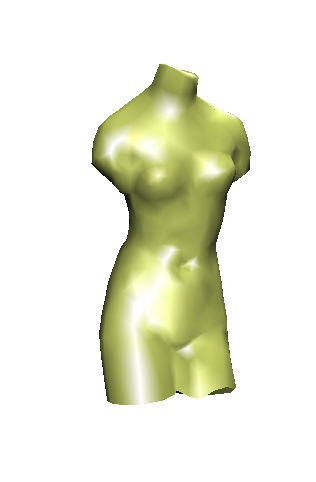
\includegraphics[width=0.3\textwidth]{figs/rbf2.png}
  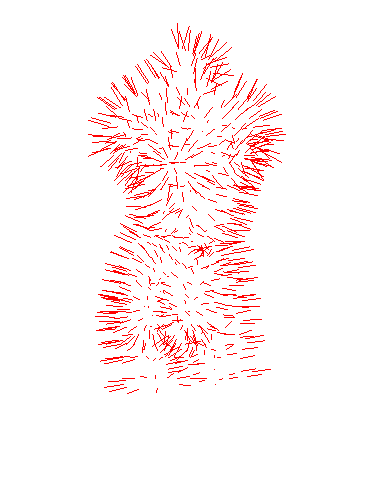
\includegraphics[width=0.32\textwidth]{figs/rbf1.png}
  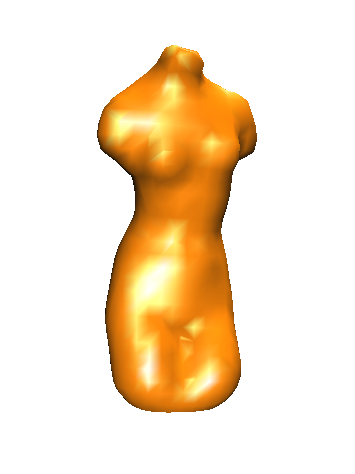
\includegraphics[width=0.32\textwidth]{figs/rbf3.png}
    \vspace{-0.75cm}
  \caption{Superfície original do modelo Venus dada por uma malha triangular (esquerda). Nuvem de pontos e normais (meio)  amostrada em 200 pontos. Superfície implícita que interpola a nuvem de pontos (direita).}
  \label{fig:rbf1}
\end{figure}  

Uma superfície implícita é definida como sendo o conjunto: 
$$ 
\mathcal{S}=f^{-1}(0)=\left\{ \mathbf{x}\in\Omega\subset\mathbb{R}^{3}:f(\mathbf{x})=0\right\}\,,
$$ 
onde $f:\Omega\subset\mathbb{R}^{3}\rightarrow\mathbb{R}$ é uma função escalar. A função $f$ é definida tal que um ponto $\mathbf{x}$ está no interior da superfície $\mathcal{S}$ tem $f(\mathbf{x}) < 0$ e quando $\mathbf{x}$ está no exterior de $\mathcal{S}$ temos $f(\mathbf{x}) > 0$. Logo, para verificar se um ponto $\mathbf{x}$ está dentro ou fora de uma superfície $\mathcal{S}$ basta observar o~sinal de $f(\mathbf{x})$. Por~outro lado, fazer amostragem de pontos sobre uma superfície implícita é um processo laborioso do ponto de vista computacional, pois se torna um problema de achar raízes de uma função não-linear. Por esse motivo a representação de superfícies implícitas se torna mais difícil do que a representação de superfícies paramétricas. Entretanto, uma maneira de contornar esse problema é recorrer ao uso de aproximações poligonais, também conhecidas como métodos de \emph{poligonização}~\cite{Abel2009}.

\medskip

O projeto proposto tem como finalidade estudar e programar técnicas que são o estado da arte em reconstrução de superfícies implícitas a partir de nuvem de pontos.
O projeto será dividido em duas etapas: poligonização e definição da superfície implícita dada por uma nuvem de pontos.

\medskip

Na primeira etapa do projeto, vamos estudar alguns algoritmos de poligonização. O processo de  poligonização de superfícies implícitas pode ser obtido através de uma decomposição espacial uniforme em células $\Omega_i$ do domínio $\Omega$, associado a uma interpolação linear dos dados amostrados ou de uma aproximação de~$f(x)$ formando uma malha composta por um conjunto de faces planares, geralmente triangulares, delimitadas por vértices e arestas. Nessa etapa adotaremos o famoso algoritmo de \emph{Marching Cubes}~ \cite{Lorensen:1987:MCA}.

\medskip

Em seguida, vamos vamos estudar um método de representação implícita de formas baseada em \emph{partição da unidade multi-nível}~\cite{CSRBF}. Esse método permite que sejam definidas superfícies implícitas a partir de grandes conjuntos de pontos (nuvem de pontos). Os principais pontos a serem estudados nessa etapa são:
%
\begin{enumerate}
\item \emph{Funções de Base Radial} que capturam a forma local da superfície de pontos através de um processo de interpolação; 

\item\emph{Partição da unidade} que é responsável por fazer uma colagem suave das funções de base radial e assim criar a superfície global;

\item \emph{Estruturas de dados espaciais} que permitam uma subdivisão hierárquica do espaço permitindo que o método se adapte de forma eficiente a geometria da superfície definida pela nuvem de pontos.
\end{enumerate}

O estudo a ser realizado nesse projeto terá como principal referência o moderno livro elaborado por Gomes~\emph{et al}~\cite{Abel2009}, além do artigo de Ohtake \emph{et al.}~\cite{CSRBF}.
%
%%%%%%%%%%%%%%%%%%%%%%%%%%%%%%%%%%

%%%%%%%%%%%%%%%%%%%%%%%%%%%%%%%%%%
\section{Justificativa} 
%%%%%%%%%%%%%%%%%%%%%%%%%%%%%%%%%%
%
O principal objetivo desse projeto é cobrir tópicos que usualmente não são abordados durante os cursos de graduação em ciência da computação.  Além disso, esse projeto pretende propiciar um maior contato do aluno com a modelagem geométrica, área de interesse do Grupo de Processamento Visual e Geométrico do ICMC-USP, tendo em vista as aplicações dessa área na indústria.
%
%%%%%%%%%%%%%%%%%%%%%%%%%%%%%%%%%%
\section{Objetivos}
%%%%%%%%%%%%%%%%%%%%%%%%%%%%%%%%%%
Este projeto de pesquisa tem a finalidade de fornecer ao bolsista condições de desenvolver sua capacidade de dedução, criatividade e raciocínio lógico na  interpretação de problemas geométricos e computacionais. Além disso, o projeto proporcionará ao aluno um maior contato da interdisciplinaridade  da matemática aplicada com outras áreas do conhecimento (Computação, Matemática e \emph{Design}, por exemplo).

\medskip
\medskip

Os objetivos específicos do projeto proposto são:  
%
\begin{enumerate}
	\item Revisar conceitos de geometria diferencial e métodos numéricos;
	\item Fazer uma revisão bibliográfica dos trabalhos relacionados;
	\item Estudar e implementar os algoritmos clássicos de reconstrução;
	\item Compreender e analisar os resultados.
\end{enumerate}
%
%
%%%%%%%%%%%%%%%%%%%%%%%%%%%%%%%%%%
\section{Metodologia}
%%%%%%%%%%%%%%%%%%%%%%%%%%%%%%%%%%
%
Nessa seção vamos descrever as ferramentas numéricas que serão utilizadas na reconstrução de uma superfície dada por uma nuvem de pontos. Na~modelagem implícita a reconstrução é dada por uma superfície implícita interpolante.
%
\subsection*{Modelagem Implícita}
%
A geração da superfície implícita será realizada usando um método de interpolação baseado em \emph{Funções de Base Radial} (\textsf{FBR})~\cite{RBF}. Uma \textsf{FBR} é uma função $W_{i}(\mathbf{x})$ que depende apenas da distância dos pontos dados aos seus \emph{centros} $\mathbf{p}_i$
$$
W_i(x) = w(||\mathbf{x}-\mathbf{p}_i||_2)\,
$$ 
onde $w(r)$ é uma função real e pode ser definida de várias formas diferentes. Exemplos de \textsf{FBR} são:

\begin{itemize}
\item{função gaussiana: $w(r) = \exp( -r^2/h^2 )$}
\item{splines poli-harmônica: $w(r) = r^k\,\mathrm{ln}(r)$ com $k=2,4,6,\ldots$}
\end{itemize}
Outros exemplos de \textsf{FBR} podem ser encontrados em \cite{RBF}. Em particular, usamos nesse projeto a função $w(r)=r$.

\begin{figure}[!ht]
	\centering
	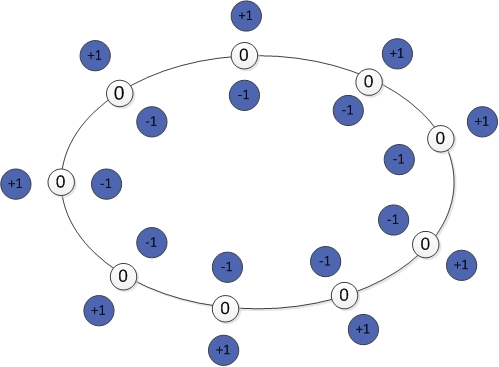
\includegraphics[scale=0.5]{figs/offset.png}
	\caption{Pontos sobre a curva a função $f(\mathbf{x})$ assume o valor 0, pontos fora da curva, ou seja, nos offsets (azul) $f(\mathbf{x})$ tem valor $-1$ se for interno ou $+1$ se for externo. }
\label{fig:offset}
\end{figure}

\bigskip{}

Dados $n$ pontos (e normais) distintos $\{\mathbf{x}_1,\mathbf{x}_2,\ldots,\mathbf{x}_n\}$, queremos obter uma superfície implícita $\mathcal{S}=f^{-1}(0)$ com $f(\mathbf{x}_i) = 0$, ou seja, $\mathbf{x}_i \in \mathcal{S}$. 
Além~de usar os pontos $\mathbf{x}_i$ como centros $\mathbf{p}_i$ de cada \textsf{FBR}, precisamos criar centros dentro e fora da superfície, pontos  conhecidos como \emph{offsets}. A Figura~\ref{fig:offset} mostra como são criados esses novos centros (offsets). Se $\mathbf{n}_i$ é a normal exterior da superfície no ponto $\mathbf{x}_i$, os pontos do offset seriam criados da seguinte maneira:
%
$$\mathbf{p}_i = \mathbf{x}_i \pm d \, \mathbf{n}_i\,,$$
%
com  $f(\mathbf{p}_{i}) = 1$, se $\mathbf{p}_i$ for ponto externo (fora da superfície) e $f(\mathbf{p}_{i}) = -1$, se $\mathbf{p}_i$ for ponto interno (dentro da superfície). O~valor~$d$ determina a largura do offset. Note que, ao criar o offset triplicamos o número de pontos iniciais.


\medskip{}

A ideia central para construir $f(\mathbf{x})$ consiste em escrever $f({x})$ como uma combinação linear das \textsf{FBR} $W_{i}(\mathbf{x})$ com $i=1,\ldots,n$:
%
$$
f(x) = \sum_{i = 1}^{n} \lambda_{i} W_{i}(\mathbf{x})\,.
$$
%
Para determinar os valores de $\lambda_i$ precisamos resolver o sistema linear $A \lambda = f$, onde $A$ é a matriz dada por:
$$A = \begin{bmatrix}
W_1(\mathbf{p}_1) & \cdots & W_1(\mathbf{p}_n) \\ 
\vdots & \ddots & \vdots \\ 
W_n(\mathbf{p}_1) & \cdots & W_n(\mathbf{p}_n)
\end{bmatrix}  
$$
%

\medskip{}
 
O método usando \textsf{FBR} apresenta alguns problemas. O número de restrições aumenta com o número de pontos, quanto maior o número de pontos maior será o consumo de memória e custo computacional. Além disso, é~difícil saber qual o melhor valor de $d$ (largura do offset), na prática é um parâmetro que depende dos dados de entrada e que para diferentes valores pode gerar superfícies com geometria e topologia distintas.

\medskip{}
 
A fim de evitar os problemas computacionais da reconstrução via \textsf{FBR}, pretendemos estudar o método proposto por Ohtake~\emph{et al.}~\cite{CSRBF} que consiste em fazer uma subdivisão hierárquica da caixa limitante da nuvem de pontos $\Omega \subset \mathbb{R}^3$ usando uma estrutura de dados conhecida como \emph{octree}~\cite{Berg:2008:CGA}. A ideia principal da octree é dividir de forma recursiva a caixa limitante da superfície em octantes.

No próximo passo, são calculadas reconstruções locais $F_{i}(\mathbf{x})$ com \textsf{FBR} de $f(\mathbf{x})$ em cada folha $\Omega_i$ da octree e em seguida uma aproximação global $f(\mathbf{x})$ é feita usando $F_{i}(\mathbf{x})$ da seguinte forma:
$$
f(\mathbf{x}) \approx \sum_i \phi_{i}(\mathbf{x}) F_{i}(\mathbf{x})\,,
$$
%
onde $\phi_i(\mathbf{x})$ são funções suaves não-negativas de suporte compacto, tais que $\sum_i \phi_{i} \equiv 1$.
Essa família de funções $\{\phi_i\}$ é chamada de \emph{partição da unidade}. Em particular, podemos definir $\phi_i(\mathbf{x})$ usando \textsf{FBR} não-negativas de suporte compacto como segue:
$$
\phi_i(\mathbf{x}) = \frac{W_i(\mathbf{x})}{\sum_{j=1}^{n} W_j(\mathbf{x})}
$$
%
Em particular, podemos escolher  $W_i$ como sendo a função Gaussiana.

%%%%%%%%%%%%%%%%%%%%%%%%%%%%%%%%%%
\section{Cronograma de Execução}
%%%%%%%%%%%%%%%%%%%%%%%%%%%%%%%%%%
%
Nesse projeto serão realizados encontros semanais com o aluno para discutir os tópicos estudados e implementados por ele. Todas as etapas do projeto serão desenvolvidas na linguagem de programação Python  e na biblioteca gráfica Matplotlib.

\medskip

A duração do projeto proposto será de 12 meses, com início previsto para Setembro de 2022. O~cronograma do projeto consiste em três etapas principais divididas da seguinte maneira:
%
\begin{enumerate}
	\item Estudo teórico e conceitual dos assuntos voltados ao projeto: 2 meses.
	\item Implementação e desenvolvimento dos códigos dos programas: 6 meses.
	\item Validação dos métodos estudados via análise dos resultados: 2 meses.
	\item Preparação do relatório final e submissão de um artigo de IC: 2 meses.
\end{enumerate}
%

%%%%%%%%%%%%%%%%%%%%%%%%%%%%%%%%%%
\section{Atividades e Resultados}
%%%%%%%%%%%%%%%%%%%%%%%%%%%%%%%%%%
\paragraph*{Detalhamento das atividades a serem desenvolvidas pelo(a) bolsista.}
O projeto tem a intenção em contar com um bolsista. A ideia é que o(a) bolsista cumpra todas as etapas do cronograma de execução do projeto, desde o desenvolvimento de um código computacional que implemente os tópicos estudados no projeto, assim como a elaboração de artigos de IC. 

\paragraph*{Resultados previstos e seus respectivos indicadores de avaliação.}
Como resultado previsto, espera-se um código computacional robusto que será disponibilizado em algum repositório público e a submissão de um artigo de IC para uma conferência da área, tais como, SIICUSP, CNMAC, SBGames, ou Sibgrapi. A relevância dessas conferências será um bom indicador de avaliação do projeto.

%%%%%%%%%%%%%%%%%%%%%%%%%%%%%%%%%%%%%%%%%%%%%%%%%%%%%%%%%%%%%%%%%%%%%%%%%%%%%%%%%
%\pagebreak
\bibliography{proj_ic}
%%%%%%%%%%%%%%%%%%%%%%%%%%%%%%%%%%%%%%%%%%%%%%%%%%%%%%%%%%%%%%%%%%%%%%%%%%%%%%%%
\end{document}
%%%%%%%%%%%%%%%%%%%%%%%%%%%%%%%%%%%%%%%%%%%%%%%%%%%%%%%%%%%%%%%%%%%%%%%%%%%%%%%%
